\documentclass[11pt, a4paper, USenglish]{article} 

\usepackage{CompendiumStyle}
\usepackage[utf8]{inputenc}

\begin{document}

% Titlepage
\title{Algorithms and Data Structures Compendium}
\author{Olav Landmark Pedersen}
\date{2018}
\begin{titlepage}
    \maketitle
    \begin{figure}
    \centering
    
\includegraphics[width=0.5\textwidth]{images/logontnu_eng.pdf}
    Department of Engineering Cybernetics
    \end{figure}
    \thispagestyle{empty}
\end{titlepage}

% TOC
\newpage
\tableofcontents
\thispagestyle{empty} % Avoid page numbering on the table of contents.

% Main content
\newpage
\setcounter{page}{1}
\section{Course Content}
See the course document to see the learning goals for each group of chapters as these are what can be tested. 
\begin{todolist}
    \item Kap. 1.  The role of algorithms in computing
    \item Kap. 2.  Getting started
    \item Kap. 3.  Growth of functions: Innledning og 3.1
    \item Kap. 4.  Divide-and-conquer: Innledning, 4.1 og 4.3–4.5
    \item Kap. 6.  Heapsort
    \item Kap. 7.  Quicksort
    \item Kap. 8.  Sorting in linear time
    \item Kap. 9.  Medians and order statistics
    \item Kap. 10. Elementary data structures
    \item Kap. 11. Hash tables: s. 253–264
    \item Kap. 12. Binary search trees: Innledning og 12.1–12.3
    \item Kap. 15. Dynamic programming: Innledning og 15.1, 15.3–15.4
    \item Kap. 16. Greedy algorithms: Innledning og 16.1–16.3
    \item Kap. 17. Amortized analysis: Innledning og s. 463–465 (tom. «at most 3»)
    \item Kap. 21. Data structures for disjoint sets: Innledning, 21.1 og 21.3
    \item Kap. 22. Elementary graph algorithms: Innledning og 22.1–22.4
    \item Kap. 23. Minimum spanning trees
    \item Kap. 24. Single-source shortest paths: Innledning og 24.1–24.3
    \item Kap. 25. All-pairs shortest paths: Innledning og 25.2
    \item Kap. 26. Maximum flow: Innledning og 26.1–26.3
    \item Kap. 34. NP-completeness
    \item Oppgaver 2.3-5, 4.5-3, 16.2-2 og 34.1-4, med løsning
    \item Appendiks A–E i dette heftet
\end{todolist}
\section{The Role of Algorithms}

\subsection{Learning goals part 1}
\begin{itemize}
    \item Chapters
    \begin{todolist}
        \item Chapter 1: The role of algorithms in computing
        \item Chapter 2: Getting Started:
            \begin{todolist}
                \item Introduction
                \item 2.1
                \item 2.2
            \end{todolist}
        \item Chapter 3: Growth of Functions:
            \begin{todolist}
                \item Introduction
                \item 3.1
            \end{todolist}
        
    \end{todolist}
        \item Goals 
    \begin{todolist}
        \item Forstå bokas pseudokode-konvensjoner
        \item Kjenne egenskapene til random-access machine-modellen (RAM)
        \item Kunne definere problem, instans og problemstørrelse
        \item Kunne definere asymptotisk notasjon
        \item Kunne definere best-case, average-case og worst-case
        \item Forstå løkkeinvarianter og induksjon
        \item Forstå rekursiv dekomponering og induksjon over delproblemer
        \item Forstå Insertion-Sort
    \end{todolist}
\end{itemize}


\section{Getting Started}

\begin{itemize}
        \item Goals 
    \begin{todolist}

        
        \item Forstå bokas pseudokode-konvensjoner
        \item Kjenne egenskapene til random-access machine-modellen (RAM)
        \item Kunne definere problem, instans og problemstørrelse
        \item Kunne definere asymptotisk notasjon
        \item Kunne definere best-case, average-case og worst-case
        \item Forstå løkkeinvarianter og induksjon
        \item Forstå rekursiv dekomponering og induksjon over delproblemer
        \item Forstå Insertion-Sort
    \end{todolist}
\end{itemize}


\section{Growth of Functions}\label{sec:GrowthOfFunctions}

\begin{equation} \label{eq1}
    \begin{split}
        f(n) & = O(g(n))   \text{     is like     }  a\leq b   \\
        f(n) & = \Omega(g(n)) \text{     is like     }   a\geq b   \\
        f(n) & = \Theta(g(n))  \text{     is like     }  a= b   \\
        f(n) & = o(g(n)) \text{     is like     }  a < b \\
        f(n) & = \omega(g(n)) \text{     is like     }  a>b  
    \end{split}
\end{equation}

\subsection{}
\section{Divide-and-Conquer}

Pensum:

Læringsmål:

\begin{itemize}
    \item Chapters
    \begin{todolist}
        \item Kap. 2. Getting started: 2.3
        \item Kap. 4. Divide-and-conquer
            \begin{todolist}
                \item Introduction
                \item 4.1
                \item 4.3
                \item 4.4
                \item 4.5
            \end{todolist}
        \item Kap. 7. Quicksort
        \item Oppgaver 2.3-5 og 4.5-3 med løsning (binærsøk)
            \begin{todolist}
                \item 2.3
                \item 2.4
                \item 2.5
                \item 4.5-3 (binary search)
                \item Appendix B and C in the syllabus
            \end{todolist}
        \item Appendiks B og C i dette heftet
    \end{todolist}
        \item Goals 
    \begin{todolist}
        \item Forstå designmetoden divide-and-conquer (splitt og hersk)
        \item Forstå maximum-subarray-problemet med løsninger
        \item Forstå Bisect og Bisect 0 (se appendiks C i dette heftet)
        \item Forstå Merge-Sort
        \item Forstå Quicksort og Randomized-Quicksort
        \item Kunne løse rekurrenser med substitusjon, rekursjonstrær og masterteoremet
        \item Kunne løse rekurrenser med iterasjonsmetoden (se appendiks B i dette heftet)
        \item Forstå hvordan variabelskifte fungerer
    \end{todolist}
\end{itemize}

\subsection{What is Divide and Conquer}
Just dividing the problem into subproblems. These subproblems should be the same as the main problem. They cannot be different problems as the main problem, but have to be broken down into smaller steps.   

The implementation of these algorithms are recursive.   

\begin{lstlisting}
    DAC(P) {
        if (small (P))
            S(P)
        else
            divide P into P1, P2, P3,...Pk
            Apply DAC(P1),DAC(P2),DAC(P2)
            Combine(DAC(P1),DAC(P2),DAC(P2)) 
       return output 
    }
\end{lstlisting}
\vspace{5mm}
 
\textbf{Functions that use Divide and Conquer}
\begin{itemize}
    \item Binary Search
    \item Finding Maximum and Minimum
    \item MergeSort
    \item QuickSort 
\end{itemize}

\subsection{Reccurence methods}

\subsubsection{Substitution}
We guess a bound and then use mathematical induction to prove our guess correct.
There are two steps:
\begin{enumerate}
    \item Guess the form of the solution
    \item Use induction to find the constants and show that the solutions works
\end{enumerate}

After making a good guess of the run time $\mathbf{T()}$ for the function. Write it out it out mathematically, and set it into the recurrence.   
Feks: \\  
\begin{itemize}
    \item With a recurrence such as  $T(n)= 2T([n/2])+n$  and you guess that the function has a run time of $O(n)$ then you would "convert" your run time guess into $cn\cdot \log(n)$ and sub it into in the recurrence and iterate through it. 
    \item For the recurrence below the run time iteration that would be smart to start with would be:
\end{itemize}
\begin{align}
     T([n/2]) &\leq c[n/2]\cdot \log([n/2]) \\
     T(n)&\leq 2(c[n/2]\cdot \log([n/2]))+n \\
     T(n)&\leq cn\cdot lg(n/2) + n \\
    &.\\
    &.\\
    &.\\
\end{align}

Eventually you will get back to the runtime that you proposed and have therefore proven that the recurrence has your runtime.\\

\emph{Changing Variables:} 
Sometimes is might be beneficial to make a substitution of a variable feks. $m=lg (n)$ and then for the runtime as well: $S(m)= 2S(m/2)+m$. Making the induction easier.

\subsubsection{Recursion-tree method}
Converts the recurrence into a tree whose nodes represent the costs incurred at various levels of the recursion. We use techniques for bounding summations to solve the recurrence. 

Start by ignoring the recursive call and put what is left over at the senter start of the tree. Feks. if your recurrence is
\begin{equation}
    T(n)= 2T([n/2])+4n
\end{equation}
Then the "root" of the tree would be $4n$. The number multiplied with $T(n)$, $2$, indicates how many iterations must be taken in the step below.
In the next iteration (step below) at each nodes, the part of the recurrence that is not a recursive call, $4n$, is then subbed into the node. However instead of $n$ the level or the call/iteration is used instead. In this case it would be $n/2$.

For each row make note of: 
\begin{itemize}
    \item Number of nodes
    \item Sum of node values
    \item Call or current iteration. 
\end{itemize}

The total numer of iterations of iterations would be the final form of the calls. In the example above it would be: $T(n/2^{i})$. To find out the number of iterations $i$, simply rearrange algebraically. 
$$ i = \log_2(n) $$
Number of iteration are used to calculate the total sum of all the row sum. 

\noindent A good example:  \href{https://www.youtube.com/watch?v=sLNPd_nPGIc}{here}
\vspace{5mm}

\subsubsection{Master's Method}
Provides bounds for currences of the form\\
\begin{equation}
    T(n) = aT(n/b)+ f(n) \qquad \text{  where  } a \geq 1,  b > 1
\end{equation}
Provides bounds for currences of the form
\begin{equation}
    T(n) = aT(n/b)+ f(n)
\end{equation}
where a $\geq$ 1, and b > 1. Then $T(n)$ has the asymptotic bounds:
\begin{enumerate}
    \item If $f(n) = O(n^{\log_b(a-\epsilon)})$ for some constant $\epsilon > 0$, then $T(n) = \Theta(n^{\log_b(a)})$ 
    \item If $f(n) = \Theta(n^{\log_b(a)})$ , then $T(n) = \Theta(n^{\log_b(a)}\cdot \log(n))$
    \item If $f(n) = \Omega(n^{\log_b(a+\epsilon)})$ for some constant $\epsilon > 0$, and if $af(n/b)\leq cf(n)$ for some constant $c<1$ then $T(n) = \Theta(f(n))$
\end{enumerate}

\subsection{Insertion Sort}
This algorithm is one of the most straight forward and slowest sorting algorithms.
It starts on the left of the algorith
\section{Dynamic Programming}

Two things that are needed for Dynamic Programming:\\

\emph{Optimal Substructure:} If an optimal solution to the problem can be constructed from optimal solutions to subproblems.\\

\emph{Overlapping Subproblems:} When a recursive algorith revisits the same problem repeatedly we say it has overlapping subproblems.\\

Divide and Conquer is not suited for problems that occur several times as this means it solves those \emph{overlapping subproblems} each time and dynamic program is a strategy to not have to recompute these problems. 

There are two main strategies of Dynamic programming.\\

\emph{Memoisation:} This strategy that is top-down idea that saves the solution to a subproblem in a data structure, and that then check up that value when you come acrosse the same subproblem again. \\

\emph{Iterative: } This is a bottom-up strategy 

\subsection{0/1 Knapsack Problem}

The 0/1 Knapsack problem is if a single object of weight and price should be included in the knapsack that can only carry a certain weight. The goal is to maximize the profit. \\

Given a price vector $p = {1, 2, 5, 6}$ and a weight vector $w = {2, 3, 4, 5}$. The solution to the problem is an vector that is binary indicating whether the object is included or not, $x = {0, 1, 0, 1}$. 
Since every item is either included or not, and all solution have to be checked the problem is $\mathcal{O}(2^n)$. This can be shortend by dynamic programming.\\

You set up a table where the columns is every weight that can be had in the bag. feks 1 - 8 for a bag that can take 8 kg. The row values are the objects in addition to having nothing in the bag. Since we are solving the problem for each step, there is a smell of optimal substructure and overlapping subproblems. 

The algorithm for this might be sligtly confusing, but just thing logically about the table. Fill the weight for each of these and put in the next object for the next weight.

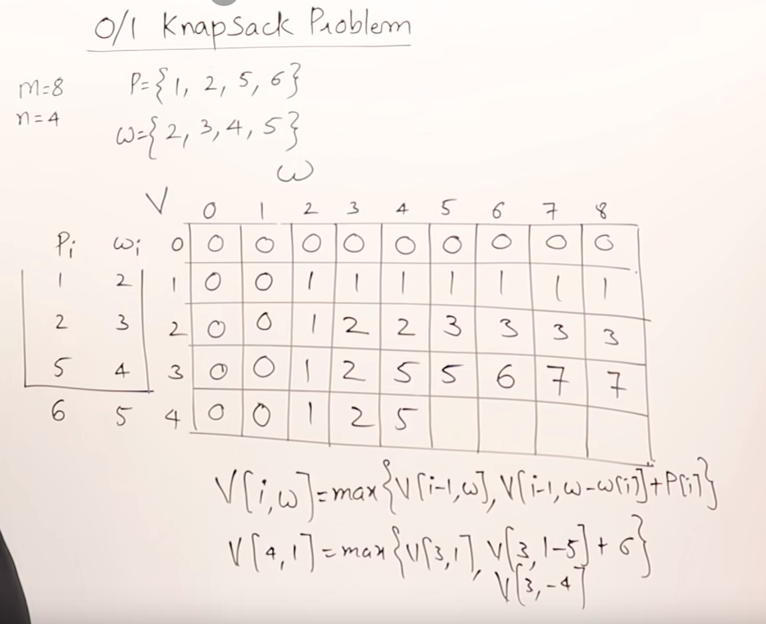
\includegraphics[width=\textwidth]{images/01Knapsack.png}

\subsection{Rod cutting}

Rod cutting problem is determining the optimal number of cuts to be done a rod. There are different prices for different lengths of the rod. You would have a length of the rod and a corresponding price $p = {1, 5, 8, 9, 10, 17, 17, 20}$. The idea is to solve the problem for each lengths $i$ of the rod and a corresponding \emph{optimal price} vector. The algorithm uses the following  to solve the problem. 

\begin{equation}
    C(i)=\max_{1\leq k \leq i}\{V_k + C(i-k)\}
\end{equation}

Where $C(i)$ is the optimal cost at index $i$, and $k$ is the number of cuts\, 
This essentially means taking the maximum previous ($C(i-k)$) and adding on the price, based on the length left over based on he price ($5$). This uses the table below and previously calculated problems to find the optimal solution. 

Without dynamic programming this problem has a solution of $\mathcal{O}(2^n)$, but with dynamic programming it reduces to $\mathcal{O}(n^2)$,

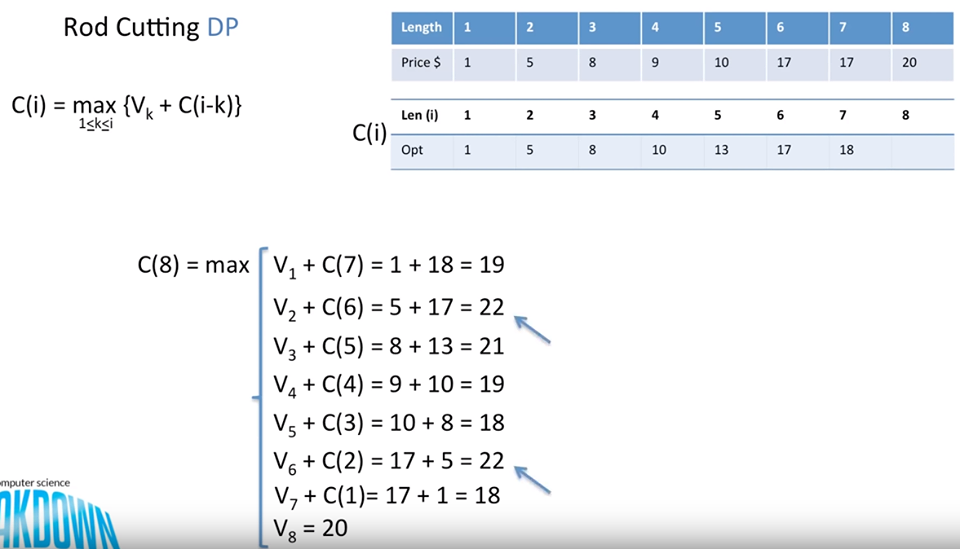
\includegraphics[width=\textwidth]{images/RodCutting.png}

\section{Greedy Programming}

There are two requirements for greedy programming:

\emph{The Greedy Choice Property} is that a global optimal solution can be arrived at by selecting a local optimmum.\\

\emph{Optimal Substructure:} If an optimal solution to the problem can be constructed from optimal solutions to subproblems.\\

\subsection{Activity Selection}

This is the problem is to choose as many activity as possible that do not overlap. In this type of problem the optimal solution is the always take the activity that finishes first relative to the ending time of the last activity. Therefore the problem is an example of a use of a greedy algorithm. 

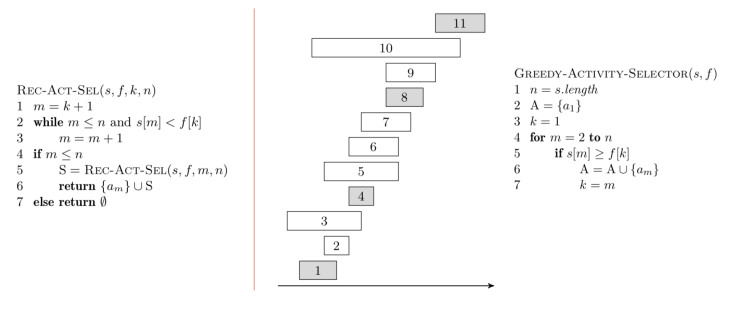
\includegraphics[width=\textwidth]{images/ActivitySelection.png}

\subsection{Huffman Coding Algorithm}

This is a compression algorithm that uses greedy programming. Remember information flow from TilpDat. 
The ideas is that you try to minimize the code, by assigning less bits to the symbol that occurs the most and more bits for those that occur less often. 

\begin{enumerate}
    \item The first step of the algorithm is to take the two characters with the lowest frequency.
    \item Then make a subtree from them and write the sum of the frequencies of both letters in the node above them.
    \item Now take the next lowest occurring symbol and set it beside the previous parent node and create a new parent node from the two. 
    \item Label the parent node with the total number of occurences in the new tree.
    \item Continue iterating through this method until the current parent node is greater than the frequency of all other nodes. 
    \item When this occurs, you need to start a new subtree with the remaining lowest frequency letters and create a parent node like we initially did.
    \item If there are remaining letters you want to take the lowest value subtree and lowest value letter and attach them together. 
    \item Finally, attach the subtrees together.
\end{enumerate}

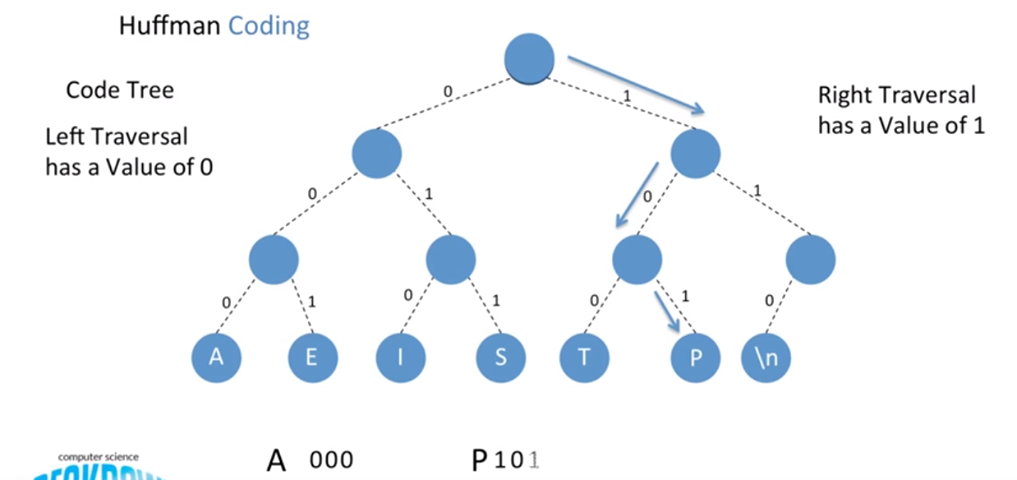
\includegraphics[width=\textwidth]{images/NonHuffman.png}

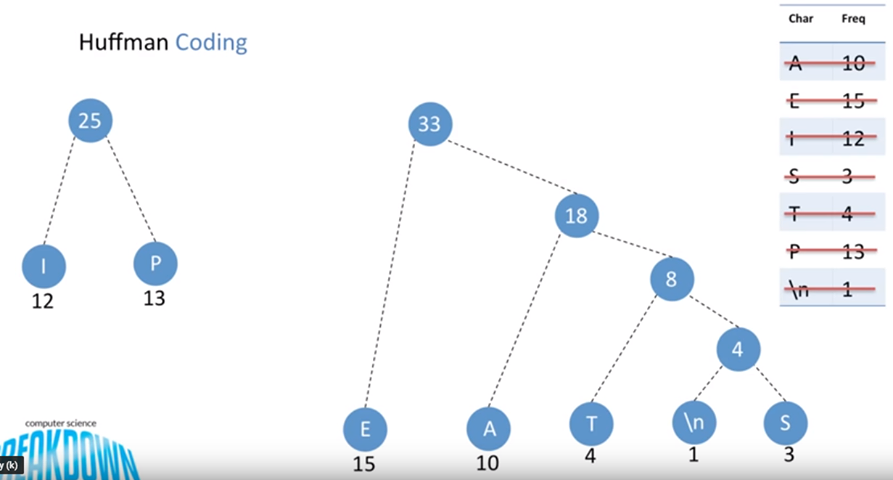
\includegraphics[width=\textwidth]{images/Huffman.png}
\section{Graphs}

Graphs are made up of 
\begin{itemize}
    \item \bf{Vertices:} Nodes or the round dots
    \item \bf{Edges:} the lines between vertices
\end{itemize}

A graph can either be \textbf{directed} or \textbf{undirected}. When making neighboring matrices or hashtabels, treat the row index as the source that the vertix point to. In undirected graphs the different just treat them like bidirectional graphs. This means that the neighbor matrices become symmetrical graphs. 

\subsection{Binary search trees}

a \emph{Successor} is the node with the smallest key, greater than the current node.
In a graph this will be the neighboring smaller value. In a normal setting this will be the right most leaf node of the LEFT branch. 
a \emph{Predecessor} is the node with the greatest key, smaller than the current node.
In a graph this will be the neighboring larger value. 
In a normal setting this will be the left most leaf node of the node on the RIGHT branch. 

\subsection{Heaps}

The way a heap is indexed in an array is that for a node $i$

\begin{align}
    \text{Left child} = 2i \\
    \text{Right child} = 2i+1
\end{align}

\textbf{The Heap Property:} The heap must have all children nodes filled, except the highest vertices. 
\part{Graph Traversal}

Notation!

\begin{table}[h!]
\centering
 \begin{tabular}{||c c||} 
 \hline
 Term & Definition \\ [0.5ex] 
 \hline\hline
 G & Graph \\ 
 V & Vertex \\
 E & Edge \\
 s & source (The node we are starting with)\\
 u & parent or predecessor vertex\\
 v & child or successor vertex\\
 u.color & This is the color attribute of the node\\
 u.d & This is the distance of the current node from the source\\
 u.$\pi$ & This is predecessor node of the node $u$ \\
 u.f & This records the \emph{time} in a DFS when the node has been blackend.\\
 Q & The queue that nodes are loaded onto. \\ [1ex] 
 \hline
 \end{tabular}
\end{table}

Color scheme

\begin{itemize}
    \item All \textbf{black} and \textbf{grey} nodes have been discovered.
    \item All \textbf{black} nodes have had all of their children nodes discovered. Note that all parent nodes, \emph{u}, are always black.
    \item All \textbf{grey} nodes might potentially have undiscovered adjacent children nodes.
\end{itemize}

\section{General Graph Traversal}

These graphs and functions are to be used on directed or undirected (or bidirectional) and non-weighted edges and are general principles for searching through these structures.

\subsection{Breadth First Search (BFS)}

Shortly put, it discovers all vertices at distance \emph{k} from \emph{s} before discovering vertices at distance $k+1$.
This algorithm uses a queue to discover new nodes and unloads them as it goes.

\subsection{Depth First Search (DFS)}

This is complementary to the BFS as this algorithm adds children vertices to the stack and continues up the tree until it reaches a leaf vertex. When it cannot go further it backtracks and tries again, until it ultimately has searched the entire tree. 

It keeps iterating down and turning vertices GRAY as it does. Each time the node is tuned gray the 'time' of discovery is set by 

\begin{equation}
    u.d = time
\end{equation}

When it it reaches the point of no return it turns the node BLACK and then records the time it was blackend by setting: 

\begin{equation}
    u.f = time
\end{equation}

As this was called recursively each node that was visited will be blackend and $u.f$ recorded recursively.

\subsection{Topological sorting}

Sorting a graph simply means that you want to ensure that a parent, $u$, comes before its child, $v$. There are two requirments for this is a DAG (Directed Acyclic Graph):

\begin{itemize}
    \item The vertices are directed
    \item The graph is \emph{acyclic}. A graph is acyclic if it cannot get stuck in a cycle between parents and children.
\end{itemize}

\emph{DAG-shortest-path()} Uses DFS to traverse through the nodes and then uses the $u.f$ blackening times of all the nodes to sort the graph into a list. 

\section{Minimal Spanning Trees}

These algorithms are performed on undirected (or bidirectional) graphs that can be cyclic, and that are weighted. They need to be weighted for the algorithms to work.

\subsection{Kruskal}

Kruskal creates a minimum spanning tree of undirected graphs with weighted edges.
The algorithm uses the edges to find a minimum spanning tree. It will go through all of the edges of nodes that are not connected. The run time for this algorithm is that of sorting the edges. It typically uses \textbf{merge sort} and therefore the compilation time will be the the time of merge sort on the edges $\mathcal{O}(E\log{E})$. 

The algorithm sorts the edges $E$ by using Merge-sort. It will add the smallest weighted vertix to the minimum spanning tree. It will keep adding the smallest edge in the and add it to the minimum spanning tree, unless the two nodes the edges connect are already in the set of connected vertices. It continues this loop until all the nodes are in the set of connected nodes. 

Kruskal is a greedy algorithm.

\subsection{Prim's Algorithm}

This algorithm basically uses BFS from a random node. It finds the smallest weighted edge that is connected to the set of connected nodes. It finds the smallest one that does not add a node that is already in the set, and adds it to the set.

\section{Shortest Path Algorithms}

The name is self explanatory, but these algorithms find the shortest path between nodes. These functions all use the $RELAX()$ function. This function will examine a parental node, child node, and a weight on the edge inbetween them. The single purpose the function is to update the $v.d$ if the current $v.d$ is higher than another parent $u.d$ and weight $w(u, v)$. 

\begin{lstlisting}[mathescape=true]
    Relax(u, v, w)
    if v.d > u.d + w(u,v)
        v.d = u.d + w(u,v)
        v.$\pi$ = u
\end{lstlisting}


\subsection{Single Source Shortest Path (SSSP)}

These types of problems exhibit \textbf{optimal substructure}. 

\subsubsection{Bellman Ford}

This function updates an array of node and the total weight needed to travel to the vertex.

\begin{enumerate}
    \item The array is initialized by setting all the weights to $\infty$.
    \item It starts by iterating through this array. For each node it checks if the vertex has nodes that it can travel to. For each of those neighboring vertices it updates the weight using $RELAX()$.
    \item It iterates through the index and updates/ $RELAX()$ at each step. 
    \item It continues looping through this array until it cannot does not change any values through the array.
\end{enumerate}

It takes at most $V-1$ iterations. The compilation time takes $\mathcal{O}(|V|*|E|)$.
Note that this algorithm can deal with negative weights as the final array can be offset by the lowest weight in the array and then sorted. 

\subsection{Dijkstra}

This functions is based on a BFS approach. It is important to note that for this algorithm there cannot be negative weights on the edges.

\begin{enumerate}
    \item It starts at the source node and relaxes all the adjacent vertices.
    \item After they have have all been relaxed it goes to its set of visited nodes and finds adjacent nodes with the smallest weight and visits that node.
    \item It relaxes all of that nodes neighboring weights and will then look at the node in the structure that is not in the set and will visit that node. (remember all unvisited vertices are $\infty$).
    \item This continues until the nodes have ultimately finds all the vertices.
\end{enumerate}

Dijkstra's shortest path can be $\mathcal{O}(V^2)$. However, if a min-priority queue with a Fibonacci heap is used the algorithm can take: $\mathcal{O}(V\log{V}+E)$

\subsection{DAG-Shortest-Path}

If it can be used it is the most efficent algorithm. The name indicates the requirements DAG = Directed Acyclic Graph. 
The algorithm topologically sorts the graph and then for each node in topological order, each of its children are relaxed. 

This algorithm has a shortest run time of $\mathcal{O}(|V|+|E|)$
% \include{Ch6_Heapsort}
% \include{Ch7_Quicksort}
% \include{Ch8_SortingLinearTime}
% \include{Ch9_MediansAndOrderStats}
% \include{Ch10_ElementaryDataStructs}
% \include{Ch11_HashTables}
% \include{Ch12_BinarySearchTrees}
% \include{Ch15_DynamicProgramming}
% \include{Ch16_GreedyProgramming}
% \include{Ch17_AmortizedAnalysis}
% \include{Ch21_DataStrutsDisjointSets}
% \include{Ch22_ElementaryGraphAlgo}
% \include{Ch23_MinimumSpanningTrees}
% \include{Ch24_SingleSourceShortestPath}
% \include{Ch25_AllPairsShortestPath}
% \include{Ch26_MaximumFlow}
% \include{Ch34_NPCompleteness}
% \include{Appendix}

 % \input simply inserts the contents of the file, while \include forces a \newpage.
% See \input vs. \include: http://tex.stackexchange.com/questions/246/when-should-i-use-input-vs-include

% References
\newpage
\addcontentsline{toc}{section}{References}
% \printbibliography{}
\label{sec:bibliography}

\end{document}